% !TeX TS-program = txs:///duck
\documentclass{standalone}
\usepackage{tikzducks}

\begin{document}
	
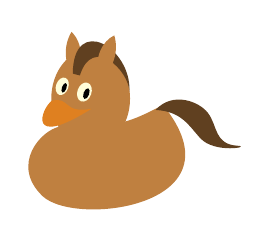
\begin{tikzpicture}

	\path (0.1,0.1) rectangle (2.7,2.4);
	\begin{pgfinterruptboundingbox}
	
		\begin{scope}[yshift=-6]
			\clip[rotate=-5] (0.68,2.38) ellipse (0.3 and 0.4);
			\fill[brown,rotate=-5](0.28,2.26)ellipse (0.3 and 0.4);
		\end{scope}
		\duck[
			body=brown,
			mohican=brown!50!black,
			horsetail
		]
		\begin{scope}[yshift=-5,xshift=1]
			\clip[rotate=-5] (0.68,2.38) ellipse (0.3 and 0.4);
			\fill[brown,rotate=-5](1.06,2.2) ellipse (0.3 and 0.4);
		\end{scope}
		
	\end{pgfinterruptboundingbox}

\end{tikzpicture}
	
\end{document}